\documentclass[11pt]{article}
\usepackage{latexsym}
\usepackage{amsmath}
\usepackage{amssymb}
\usepackage{amsthm}
\usepackage{cleveref}
\usepackage{epsfig}
\usepackage[tight]{subfigure}
\usepackage{comment}

% TD (Nitish)
%   online policy evaluation
%   learning rate, intuition and bounds (Mike)
% SARSA (Nitish)
%   define the loss function
%   derive the full gradient 
%   drop the extra term
%   explain that this is NOT gradient descent
%   mention the Bellman-Residual method
% Q-Learning (Mike)
%   online fitted Q-iteration
%   restate the parameter update
%   exploration policies: epsilon-greedy and Boltzman
% Off-Policy vs On-Policy learning (Mike)
% Experience Replay (Mike)


%extra packages added
%\usepackage{algorithm}
%\usepackage{algorithmic}
\numberwithin{equation}{section}
\numberwithin{figure}{section}
\DeclareMathOperator*{\argmax}{arg\,max}
\DeclareMathOperator{\uniform}{uniform}

\newcommand{\handout}[5]{
  \noindent
  \begin{center}
  \framebox{
    \vbox{
      \hbox to 5.78in { {#1} \hfill #2 }
      \vspace{4mm}
      \hbox to 5.78in { {\Large \hfill #5  \hfill} }
      \vspace{2mm}
      \hbox to 5.78in { {\em #3 \hfill #4} }
    }
  }
  \end{center}
  \vspace*{4mm}
}

\newcommand{\lecture}[5]{\handout{#1}{#2}{#3}{#4}{#5}}

\newtheorem{theorem}{Theorem}
\newtheorem{corollary}[theorem]{Corollary}
\newtheorem{lemma}[theorem]{Lemma}
\newtheorem{observation}[theorem]{Observation}
\newtheorem{proposition}[theorem]{Proposition}
\newtheorem{definition}[theorem]{Definition}
\newtheorem{claim}[theorem]{Claim}
\newtheorem{fact}[theorem]{Fact}
\newtheorem{assumption}[theorem]{Assumption}

% 1-inch margins, from fullpage.sty by H.Partl, Version 2, Dec. 15, 1988.
\topmargin 0pt
\advance \topmargin by -\headheight
\advance \topmargin by -\headsep
\textheight 8.9in
\oddsidemargin 0pt
\evensidemargin \oddsidemargin
\marginparwidth 0.5in
\textwidth 6.5in

\parindent 0in
\parskip 1.5ex

%\renewcommand{\baselinestretch}{1.25}

\begin{document}

%%%%%%%%%%%%%%%%%%%%%%%%%%%%%%%%%%%%%%%%%%%%%%%%%%%%
% Document header: change the lecture number, date, scribe name, and
% lecture topic.
%%%%%%%%%%%%%%%%%%%%%%%%%%%%%%%%%%%%%%%%%%%%%%%%%%%%
%\lecture{Statistical Techniques in Robotics (16-831, F10)}
%{Lecture\#NN (Thursday August 26)}
%{Lecturer: Drew Bagnell}
%{Scribe:YOUR\_NAME\_HERE \footnotemark}
%{Lecture Topic}

\lecture{Statistical Techniques in Robotics (16-899, S14)}%
{Lecture \#09, (Feb. 11, 2014)}%
{Lecturer: Drew Bagnell}%
{Scribes: Michael Koval and Nitish Thatte}%
{Q-Learning}

% Be sure to acknowledge all previous scribes.
\footnotetext[1]{Some content adapted from previous scribe: Jackie Libby}

%%%%%%%%%%%%%%%%%%%%%%%%%%%%%%%%%%%%%%%%%%%%%%%%%%%%
% Document body: Scribe your notes here.
%%%%%%%%%%%%%%%%%%%%%%%%%%%%%%%%%%%%%%%%%%%%%%%%%%%%

\section{Overview}
We have already covered several offline methods such as Fitted Value Iteration,
Fitted Q-Iteration, and Approximate Policy Iteration.  Offline methods make
efficient use of available training data, but are computationally expensive and
suffer from high memory consumption as the number of experiences increases. In
this lecture, we present several online techniques that perform well even when
presented with large amounts of data. Online methods perform an incremental
update after state transition, as shown below:

\begin{figure}[h!]
	\centering
	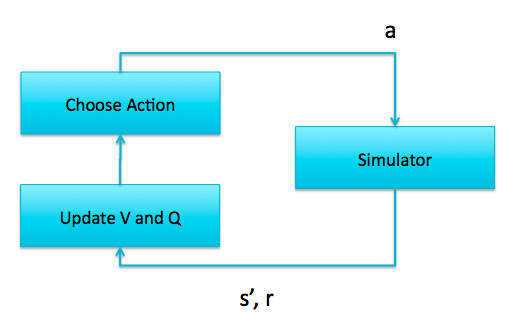
\includegraphics[width=.4\columnwidth]{./images/figBlock}
	%\caption{}
	\label{fig.figBlock}
\end{figure}

First, we will present the Temporal Differencing (TD) method for online policy
evaluation. Next, we show how SARSA extends online policy evaluation to the
action-value function. Finally, we explore Q-learning as an method of finding
the optimal policy.

\section{Temporal Differencing (TD)}
Temporal differencing, or TD-learning, is an online method of estimating the
value function
\begin{equation}
	V^\pi(s) = \sum_{t = 0}^\infty \gamma^t E\left[ r(s_t,\pi(s_t)) \right]
	\label{eq.policyEval}
\end{equation}
of policy $\pi$, where samples $s_t$ are drawn from the transition model while
following policy $\pi$.

Given an estimate of the value function $\tilde{V}^\pi(s)$ we would like to
perform an update in order to minimize the squared loss
\begin{equation}
	\mathcal{L} = \frac{1}{2} \left(V^\pi(s) - \tilde{V}^\pi(s) \right)^2.
	\label{eq.valLoss}
\end{equation}

Since we do not yet know the value function, evaluating this loss requires
evaluating equation~\ref{eq.policyEval}. Na\"{i}vely, this method would require
waiting until the end of an episode before updating $\tilde{V}^\pi(s)$. Instead,
we estimate $V^\pi(s)$ as $y = r + \gamma \tilde{V}^\pi(s')$ and perform an
incremental update for each experience $(s, r, s')$,

Plugging this estimate into the loss function we get
\begin{equation}
	\mathcal{L} = \frac{1}{2} \left(y - \tilde{V}^\pi(s) \right)^2.
	\label{eq.valLossApprox}
\end{equation}

The derivative of \cref{eq.valLossApprox} is:
\begin{equation}
    \nabla_{\tilde{V}^\pi}\mathcal{L} = \left(y - \tilde{V}^\pi(s) \right) \left(\nabla_{\tilde{V}^\pi} y - 1 \right).
    \label{eq.valGrad}
\end{equation}

It is, unfortunately, not possible to get unbiased estimates of both
$\tilde{V}_\pi(s)$ and $y$ with only one $(s,r,s')$ tuple. To avoid this issue,
the TD method ignores the $\nabla_{\tilde{V}^\pi} y$ and uses the following update
rule:
\begin{align}
    \tilde{V}^\pi(s) &\leftarrow  \tilde{V}^\pi - \alpha \nabla_{\tilde{V}^\pi}\mathcal{L} \notag \\
                     &\leftarrow  \tilde{V}^\pi + \alpha \left(r + \gamma \tilde{V}^\pi(s') - \tilde{V}^\pi(s) \right) \notag \\
                     &\leftarrow  (1 - \alpha) \tilde{V}^\pi(s) + \alpha \left(r+ \gamma \tilde{V}^\pi(s') \right). 
    \label{eq.valUpdate}
\end{align}

\subsection*{Algorithm TD:}
\begin{enumerate}
	\item Initialize $\tilde{V}^\pi$
	\item $\forall s$, repeat until $\tilde{V}^\pi(s)$ converges
	\begin{enumerate}
		\item Initialize $s$
		\item Repeat until $s$ is terminal (This is a trajectory from a particular intitial starting state.)
		\begin{enumerate}
			\item Do $\pi(s)$
			\item Observe $s', r$
			\item Update $\tilde{V}^\pi(s)$ given  $(s, r, s')$
			\label{step.updateTD}
			\item $s \leftarrow s'$
		\end{enumerate}		
	\end{enumerate}		
\end{enumerate}		

\subsection*{Grid-World Example}
The diagram below shows a grid-based world, where the robot starts in the upper left, and the goal is in the lower right.  The robot gets a reward of $+1$ if it reaches the goal, and $0$ everywhere else.  There is a discount factor of $\gamma$.  The policy is for the robot to go right until it reaches the wall, and then go down.
\begin{figure}[h!]
	\centering
	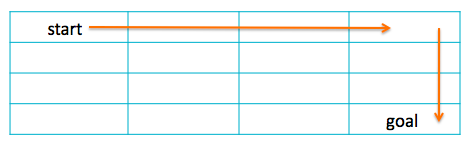
\includegraphics[width=.4\columnwidth]{./images/fig1}
	%\caption{}
	\label{fig.fig1}
\end{figure}

We start by initializing all states to 0:

\begin{figure}[h!]
	\centering
	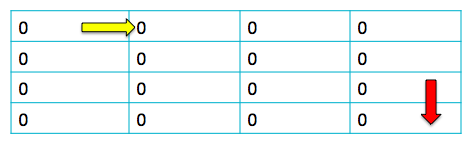
\includegraphics[width=.4\columnwidth]{./images/fig2}
	%\caption{}
	\label{fig.fig2}
\end{figure}

As the robot moves one cell over from the start state (yellow arrow above), the reward is $0$, and the value of both the current state and the next state is $0$, so the gradient used in the update rule (\cref{eq.valUpdate}) evaluates to $0$ and no update is performed. As the robot moves into the goal state (red arrow), the reward is $1$, so the gradient evaluates to $1$.  We then update the second-to-last cell with \cref{eq.valUpdate} and we get:

\begin{figure}[h!]
	\centering
	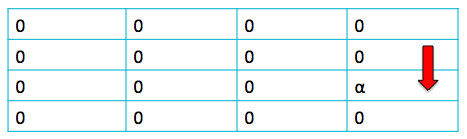
\includegraphics[width=.4\columnwidth]{./images/fig3}
	%\caption{}
	\label{fig.fig3}
\end{figure}

Another iteration of the algorithm gives us:

\begin{figure}[h!]
	\centering
	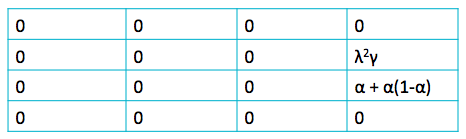
\includegraphics[width=.4\columnwidth]{./images/fig4}
	%\caption{}
	\label{fig.fig4}
\end{figure}

This method is slow, because we have to run the whole policy just to update the next cell.  
%%%%%%%%%%%%%%%%%%%%%%%%%%%%%%%%%%%%%%%%%%%%%%%%%%%%

\section{SARSA}
%%%%%%%%%%%%%%%%%%%%%%%%%%%%%%%%%%%%%%%%%%%%%%%%%%%%
SARSA extends the Temporal Differencing method presented in the previous
section to evaluate policies represented by a state-action functions
$Q^\pi(s,a)$. Similar to the TD case, we wish to evaluate a policy by
performing an online update to obtain an estimate, $\tilde{Q}^\pi(s,a)$, of the
true state-action function $Q^\pi(s,a)$:
\begin{equation}
	Q^\pi(s,a) = r(s,a) + \sum_{t = 1}^\infty \gamma^t E[r(s_t,\pi(s_t))]
	\label{eq.sarsaEval}
\end{equation}

As in TD, we seek to minimize the loss
\begin{equation}
	\mathcal{L} = \frac{1}{2} \left(y - \tilde{Q}^\pi(s,a) \right)^2
	\label{eq.sarsaLoss}
\end{equation}
where $y = r(s,a) + \gamma \tilde{Q}^\pi(s',\pi(s'))$. Following a similar
derivation as used for the TD update, we arive at the SARSA update rule:
\begin{equation}
    \tilde{Q}^\pi(s,a) \leftarrow  (1 - \alpha) \tilde{Q}^\pi(s,a)
        + \alpha \left[ r(s,a) + \gamma \tilde{Q}^\pi(s',\pi(s')) \right].
	\label{eq.sarsaUpdate}
\end{equation}
\subsection*{Algorithm SARSA:}
\begin{enumerate}
	\item Initialize $Q^\pi$
	\item Repeat until $Q^\pi$ converges
	\begin{enumerate}
		\item Initialize $s$, $a \sim \hat{\pi}_{Q(s)}$

		(This means we initialize the action randomly according to some distribution $\hat{\pi}_{Q(s)}$.)
		\item Repeat until $s$ is terminal
		\begin{enumerate}
			\item Do $a$
			\item Observe $s'$, $r$
			\item Pick $a' \sim \hat{\pi}_{Q(s')}$
			\item Update $Q^\pi(s,a)$ given $(s, a, r, s', a')$
			
			(This is where SARSA comes from!)
			\item $s \leftarrow s'$, $a \leftarrow a'$ 
		\end{enumerate}
	\end{enumerate}
\end{enumerate}

\section{Q-Learning}
Q-Learning attempts to learn the optimal action-value function $Q(s, a)$ from
an online stream of experiences. Suppose we receive experience $(s, a, r, s')$
with the approximate action-value function $\tilde{Q}(s, a)$. Performing a
Bellman backup would update the action-value function
\begin{align*}
    \tilde{Q}^*(s, a) \gets r + \gamma \max_{a' \in A} \tilde{Q}^*(s', a').
\end{align*}

However, just as in SARSA, this performs poorly when the transition or reward
functions are stochastic. Instead, we update $\tilde{Q}^*$ to the weighted sum
\begin{align*}
    \tilde{Q}^*(s, a) \gets \alpha \left[r + \gamma \max_{a' \in A} \tilde{Q}^*(s', a')\right]
                            + (1 - \alpha) \tilde{Q}^*(s, a)
\end{align*}
where $0 \le \alpha \le 1$ is the \emph{learning rate} parameter.

Q-learning is guaranteed to converge $\tilde{Q}^*$ to the optimal action-ovalue
function $Q^*$ as $t \to \infty$ given that the following conditions hold:
\begin{enumerate}
    \item Each state-action pair is visited infinite times
    \item $\lim_{t \to \infty} \sum_{t = 0}^\infty \alpha_t = \infty$
    \item $\lim_{t \to \infty} \sum_{t = 0}^\infty \alpha_t^2 < \infty$.
\end{enumerate}
The latter two conditions mean that the learning rate $\alpha$ must be annealed
over time. Intuitively, this means that the agent begins by quickly updating
$\tilde{Q}^*$, then slows down to refine its estimate as it receives more
experience.

\subsection{Fitted Q-Learning}
Just as the fitted Q-iteration algorithm, we can use a function approximator to
approximate the action-value function. Suppose that we approximate $Q$ with the
the function $\tilde{Q}^\theta$ with hyperparameter $\theta$. Instead of
directly updating our action-value function, we now must update $\theta$ to
achieve the desired change in $\tilde{Q}^\theta$.

To fit $\theta$, we minimize a loss function
\begin{align*}
    \mathcal{L} &= \frac{1}{2} \left( y - Q^\theta(s, a) \right)^2
\end{align*}
that penalizes deviation between the approximate action-value function
$Q^\theta(s, a)$ and the value $y = r + \gamma \max_{a' \in A} Q^\theta(s',
a')$ predicted by a Bellman backup. We will now find the optimal parameter
$\theta$ by performing gradient descent on $\mathcal{L}$ with the update rule
\begin{align}
    \theta &\gets (1 - \alpha) \theta + \alpha \nabla_\theta \mathcal{L}
    \label{eqn:qlearning-step}
\end{align}

First, we must derive the gradient of $\mathcal{L}$. By applying the chain
rule, we find
\begin{align*}
    \nabla_\theta \mathcal{L} &= \left(y - Q^\theta(s, a)\right) \left[
                                      \nabla_\theta y
                                    - \nabla_\theta Q^\theta(s, a) \right] \\
                              &= \left(y - Q^\theta(s, a)\right) \left[
                                      \gamma \nabla_\theta Q^\theta(s, a^*)
                                    - \nabla_\theta Q^\theta(s, a) \right]
\end{align*}
where $a^* = \argmax_{a \in A} Q^\theta(s, a)$ is the optimal action according
to $Q^\theta$. Unfortunately, it is not possible to obtain an unbiased estimate
of $Q^\theta(s, a) Q^\theta(s, a^*)$ using one sample $(s, a, r, s')$. Instead,
Q-learning assumes that $y$ is constant and approximates the gradient as
\begin{align}
    \nabla_\theta \mathcal{L}_\text{approx} &= -\left(y - Q^\theta(s, a)\right)
                                       \nabla_\theta Q^\theta(s, a).
    \label{eqn:qlearning-gradient}
\end{align}

The complete fitted Q-learning update rule is found by substituting
\cref{eqn:qlearning-gradient} into \cref{eqn:qlearning-step}:
\begin{align*}
    \theta &\gets (1 - \alpha) \theta - \alpha \left[
                y - Q^\theta(s, a)\right] \nabla Q^\theta (s, a) \\
           &\gets (1 - \alpha) \theta - \alpha \left[
                \left( r - \gamma Q^\theta(s, a^*) \right)
                - Q^\theta(s, a)\right] \nabla Q^\theta (s, a).
\end{align*}

\subsection{Bellman Residual Method}
Q-learning as described above does not implement gradient descent and, thus, is
not guaranteed to converge to a local minimum. The \emph{Bellman residual
algorithm} method avoids the approximation of \cref{eqn:qlearning-gradient} by
estimating the true gradient $\nabla_\theta \mathcal{L}$. This estimation is
only unbiased if we can generate two independent successor states for taking
action $a$ in state $s$.

Generating these samples is trivial if we are able to simulate the system; i.e.
have access to a known or learned transition model. If we do not know the
transition model, then it is only possible to perform a Bellman residual update
if we postpone a backup until the same state-action pair has been observed two
or more times. This is often impossible when learning on a real system that has
a continuous state-action space.

% TODO: Cite: http://www.leemon.com/papers/1995b.pdf

\subsection{Exploration Policies}
Unlike SARSA, which is an \emph{on-policy} method,  Q-learning is an
\emph{off-policy} method that can learn from arbitrary $(s, a, r, s')$
experiences, regardless of what policy was used to generate them. This means
that it is possible to use an \emph{exploration policy} training that
encourages the agent to visit previously unexplored regions of the state-action
space. Exploration policies guarantee that the agent visites each state an
infinite number and insures convergence in domains where an exact update is
possible.

Two exploration policies that are commonly used with Q-learning are:
\begin{enumerate}
    \item \textbf{$\epsilon$-Greedy}. Choose the greedy action $a = \argmax_{a
        \in A} Q(s, a)$ with probability $1 - \epsilon$. Otherwise, with probability
        $\epsilon$, choose an action uniformly at random $a \sim \uniform(A)$. Higher
        values of $\epsilon$ encourage more exploration.
    \item \textbf{Boltzmann Exploration.} Choose action $a$ with probability
        \begin{align*}
            p(a) = \frac{\exp\left[ \beta Q(s, a) \right]}
                        {\sum_{a' \in A} \exp\left[ \beta Q(s, a') \right]},
        \end{align*}
        which is weighted towards selecting actions with higher $Q$-values. Lower
        values of $\beta$ encourage more exploration.
\end{enumerate}

\section{Experience Replay}
Q-learning and SARSA are both computationally efficient, but make inefficient
use of data. Unlike batch methods, each sample is only used exactly once. This
means that the agent must observe each transition $(s, a, s')$ many times to
propagate the reward backwards in time.

\emph{Experience replay} allows online algorithms to re-use experience multiple
times by buiding a database $D$ of experiences.  Once enough data has been
collected, the agent performs a fixed number of Q-learning or SARSA updates on
the batch. This technique bridges the gap--and can potentially combine the
advantages of---offline and online algorithms.
\end{document}
